\documentclass{llncs}
\usepackage{afterpage}
\usepackage{enumitem}
\usepackage{mathtools}
\newcommand{\distance}{2cm}
\usepackage[left=\distance,right=\distance,top=\distance,bottom=\distance]{geometry}
\usepackage{tikz}
\usetikzlibrary{arrows.meta, positioning} 
\usepackage{hyperref}
\usepackage{listings}
\usepackage{xcolor}
\definecolor{backcolour}{rgb}{0.95,0.95,0.95}

\lstdefinestyle{mystyle}{
    basicstyle=\small\linespread{1}\selectfont,
    backgroundcolor=\color{backcolour}, 
    frame=single,
    rulecolor=\color{black},
    captionpos=b,
    numbers=left,
    numberstyle=\tiny\color{gray},
    xleftmargin=5mm,
    xrightmargin=0mm,
    aboveskip=0mm,
    belowskip=0mm,
    breaklines=true,
    abovecaptionskip=1mm,
    belowcaptionskip=2mm,
    numberbychapter=false,
}
\lstset{style=mystyle}

\begin{document}
\pagestyle{plain}

\title{Train Scheduling in Flatland via Logic Programming}
\author{Felix Marc Kratzsch}
\authorrunning{F. Kratzsch}
\institute{Potsdam University}
\maketitle
\begin{multicols*}{2}
    
\begin{figure*}[t]
\begin{minipage}[t]{0.32\textwidth}
    \centering
    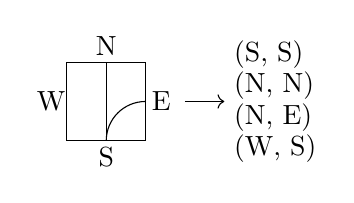
\begin{tikzpicture}
        \draw (0,0) rectangle (1,1);
        \draw[->] (1.5,0.5) -- (2,0.5);
        
        \node at (0.5, 1.2) {N};
        \node at (0.5, -0.2) {S};
        \node at (1.2, 0.5) {E};
        \node at (-0.2, 0.5) {W};
        
        \draw (0.5, 0) -- (0.5, 1);
        \draw (0.5, 0) to[out=90,in=180] (1, 0.5);
        
        \node[anchor=west] at (2, 1.1) {(S, S)};
        \node[anchor=west] at (2, 0.70) {(N, N)};
        \node[anchor=west] at (2, 0.30) {(N, E)};
        \node[anchor=west] at (2, -0.1) {(W, S)};
    \end{tikzpicture}
    \caption{Transitions}
    \label{fig:transition}
\end{minipage}
\begin{minipage}[t]{0.32\textwidth}
    \centering
    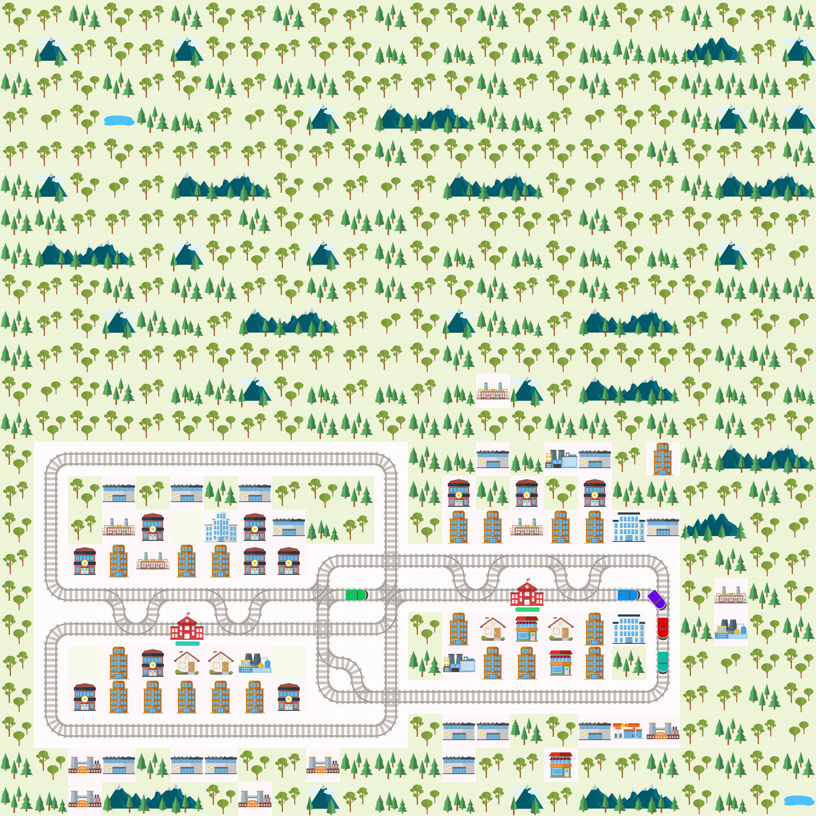
\includegraphics[width=1\textwidth,trim={0 1.3cm 3.7cm 14.4cm},clip]{images/map.png}
    \caption{Map}
    \label{fig:map}
\end{minipage}
\begin{minipage}[t]{0.32\textwidth}
    \centering
        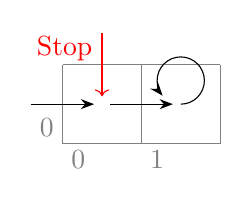
\begin{tikzpicture}
            \draw[step=1cm, gray] (0,0) grid (2,1);
            \draw[gray] (-0.2,0.2) node{0};
            \draw[gray] (0.2,-0.2) node{0};
            \draw[gray] (1.2,-0.2) node{1};
            \draw[-{Stealth}] (-0.4,0.5) -- (0.4,0.5) node[midway, above] {};
            \draw[-{Stealth}] (0.6,0.5) -- (1.4,0.5) node[midway, above] {};
            \draw[->,color=red] (0.5,1.4) -- (0.5,0.6) node[near start, left] {Stop};
            \draw[-{Stealth}] (1.5,0.5) arc(90:400:-0.3);
        \end{tikzpicture}
    \caption{Delay}
    \label{fig:delay}
\end{minipage}
\end{figure*}

\begin{abstract}
Train scheduling is a modern-day problem with many applications. The search for efficient and correct solutions is a broad field, where many approaches were presented.

This work focuses on solving train scheduling problems with logic programming and the steps taken to implement them. Herein, different approaches to transforming the problem domain are explained in concept and evaluated. The most effective approach deals with the reduction of the problem domain, but no single best approach could be determined.
\end{abstract}

\section*{Introduction}
Train scheduling is an important modern-day problem and its applications are bound to increase due to growing demands on rail networks. The problem scales across many dimensions, such as rail network size, number of trains, and varying requirements. Such requirements might be the flow of passengers or handling malfunctions. Whatever the exact specifications may be, efficient solutions are required to make automated scheduling feasible.\\

This paper uses answer set programming (ASP), as it is expressive enough to model the scheduling problem presented here, while remaining easy to understand and implement.

The railway domain used is a subset of Flatland, an environment for implementing and testing train scheduling problems. It was chosen since it provides many tools to generate maps and test solutions.\\

The goal of this work is to implement different approaches in logic programming to efficiently generate plans for train scheduling problems. To that end, a basic approach is implemented as a baseline, followed by four potential improvements.

One of them focuses on reducing the size of the rail network by removing redundancy and combining railway sections. Another one focuses on reducing computation per train by removing duplicate computation. The other two improvements focus on the logic-programming-specific problem of requiring discrete time points, instead of modelling time continuously. As train scheduling requires detailed plans, especially to avoid conflicts, a high resolution of time points is necessary. Therefore, the number of time points forms another dimension, which impacts efficiency. One improvement will focus on reducing the necessary time points, while the other implements an abstract representation to remove time points altogether.\\

In sections 2 to 5, I am going to explain the Flatland domain, describe logic programming (specifically Clingo), and explain the different approaches. Sections 6 to 8 will evaluate, discuss and summarize the results.

\section*{Related Works}
Solutions to this particular domain have been proposed for a long time. One of the more exhaustive explanations of the domain is provided by \cite[Daduna and Pinto Paix{\~a}o 1995]{Daduna1995}. 

There are many approaches, but logic programming ones are more relevant for this work. \cite[Abels et al. 2020]{Abels20} and \cite[Behrens et al. 2023]{Behrens2023} are prime examples of using logic programming. Both explicitly deal with transformations and abstractions to improve solvability in logic programming.

While the website itself provides extensive documentation \cite{Flat24}, papers specifically using Flatland with different solution strategies exist as well. \cite[Mohanty et al. 2020]{Mohanty20}, for example, describes different strategies for solving the problem, with reinforcement learning being one of them.

\section*{Flatland Domain}
Flatland \cite{Flat24} is a railway environment developed by AIcrowd. The domain provided is a simple grid environment with many extensions such as trains of differing speeds, malfunctions for rescheduling scenarios, earliest departure and latest arrival times. Furthermore, it provides tools for generating, running, and visualizing instances (maps) in the form of a Python package.\\

The grid of Flatland is mostly empty (see Figure \ref{fig:map}). Only cells with rails are represented and called transitions by Flatland. A transition consists of a cell, an entry and an exit direction. As shown in Figure \ref{fig:transition}, the possibility of moving from south to north is encoded as $(N,N)$, as the train enters and leaves facing north. In this example, the cell would be encoded as four transitions.

Flatland utilizes timesteps to measure time. In the simplest scenario (every train has the same speed), every move of one cell takes exactly one timestep. These timesteps are also used to implement the earliest departure and latest arrival times (hereafter called start times and horizons), which can vary for all trains and represent a timetable.

Every train is assigned a start and a goal. Goals are limited to cities (the red buildings on the track (seen in Figure \ref{fig:map})) and starts to cells parallel to cities (in the example the rails directly above the cities). Cities are scattered sparsely over the map, as they require a minimum distance between them. Starts, goals, timetables, as well as the initial facing direction are specified per train at instance generation.

Flatland processes plans per timestep, accepting one action for every train each timestep. The possible actions are \texttt{left}, \texttt{forward}, \texttt{right} and \texttt{stop}. The actions change the state of the train. Therefore, a \texttt{stop} action will continue until another action is given. All other actions (left, right and forward) are continued, after their direct effect, by following the rails until another action is given (hereafter called automatic movement). In this case, a train will continue moving by picking the only choice possible or moving forward.

Instead of being permanently present, trains need to be spawned in order to start the plan execution and disappear when reaching their goals. Spawning can be done with any action. A train can be spawned at its defined starting position and facing direction, but only after the current timestep has reached its earliest departure time.

Trains are not allowed to occupy the same cell at the same timestep (hereafter called vertex conflict) or exchange cells in adjacent timesteps (hereafter called swap conflict).\\

This environment is enough for the approaches presented in this work. As further features, such as different speeds or malfunctions, would complicate implementation and presentation, I decided against using them.\\

While the Flatland domain provides ease of use, there is some weird behavior (or corner/edge cases) to be aware of.

The most prominent one is the execution delay. As seen in Figure \ref{fig:delay}, a train (at $(0,0)$) receiving the action to stop, executes the action in the next timestep (after moving to $(1,0)$). This can be understood as a delay affecting all actions. Thus, a train spawned with an action would appear two timesteps later instead of one. This explanation models the behavior perfectly, but the proper explanation lies in the way Flatland models train states. If given a \texttt{stop} action, a train continues moving and sets its state to \texttt{stopped} and vice versa for starting to move. To explain this behavior for every action combination is very complicated, but as a delay explains it accurately, I will not explain it further.

It should be noted, that an action spawning a train has its immediate effect replaced by the act of spawning. It does not matter, which action is given, as long as it is a defined one. The train continues with automatic movement until a \texttt{stop} action is given. This automatic movement is not limited to the actions \texttt{left}, \texttt{forward}, or \texttt{right}. The train also starts the automatic movement if it is spawned with a \texttt{stop} action. Therefore, if waiting at the spawn is required, an action to spawn the train needs to be followed by a \texttt{stop} action to make it wait instead of moving automatically. Also, it has to be noted that the earliest departure times refer to the earliest time an agent may receive an action, not when it may spawn.

The grid alignment is unusual, but for debugging it's important to note that $(0,0)$ is the top leftmost cell, while $(1,0)$ is directly south and $(0,1)$ is directly east. As it is given by Flatland, I am going to use this alignment in this work.

Lastly, horizons set by Flatland's timetables are not always perfectly solvable. Flatland uses the shortest path as a minimum difference for generating departure and arrival times, but does not account for possible conflicts. It is therefore possible to rarely generate unsolvable instances with multiple trains.\\

Flatland provides additional tools. The visualizer (seen in Figure \ref{fig:map}) can be used to visualize plan execution, which is useful for debugging. However, it illustrates Flatland's interpretation of actions, which slightly differs from the delay explanation provided above. This can be ignored, as the underlying behavior does not change. Another tool, the instance generator, is useful to bulk generate random instances with set requirements (e.g., size, number of cities, number of trains), which is perfect for benchmarks.

\section*{Answer Set Programming}
\begin{figure*}[t]
    \begin{minipage}[b]{0.26\textwidth}
        \centering
        \scalebox{0.63}{
        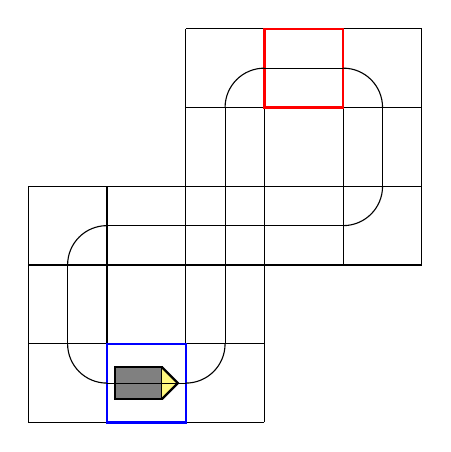
\begin{tikzpicture}
            \draw[step=1] (0,0) grid (3,3);
            \draw[step=1] (1.998,1.998) grid (5,5);

            \draw[thick, fill=black!50] (1.1,0.3) -- (1.7,0.3) -- (1.7,0.7) -- (1.1,0.7) -- cycle;
            \draw[thick, fill=yellow!50] (1.7,0.7) -- (1.9,0.5) -- (1.7,0.3);
            
            \draw[blue, thick] (1,0) rectangle (2,1);
            \draw[red, thick] (3,4) rectangle (4,5);

            \draw[color=black] (1,0.5) -- (2,0.5);
            \draw[color=black] (0.5,1) -- (0.5,2);
            \draw[color=black] (2.5,1) -- (2.5,4);
            \draw[color=black] (1,2.5) -- (4,2.5);
            \draw[color=black] (3,4.5) -- (4,4.5);
            \draw[color=black] (4.5,3) -- (4.5,4);

            \draw[color=black] (0.5,1) to[in=180,out=270] (1,0.5);
            \draw[color=black] (2,0.5) to[in=270,out=0] (2.5,1);
            \draw[color=black] (0.5,2) to[in=180,out=90] (1,2.5);
            \draw[color=black] (4,2.5) to[in=270,out=0] (4.5,3);
            \draw[color=black] (2.5,4) to[in=180,out=90] (3,4.5);
            \draw[color=black] (4.5,4) to[in=0,out=90] (4,4.5);
        \end{tikzpicture}
        }
        \caption{Example}
        \label{fig:example}
    \end{minipage}
    \begin{minipage}[b]{0.72\textwidth}
        \lstinputlisting[caption=Secondary Atoms, label={lst:input}]{listings/input.lp}
    \end{minipage}
\end{figure*}

Answer Set Programming (ASP) is a declarative approach to programming. In ASP, logical constraints are specified via predicate logic and stable models (valid truth assignments that satisfy all constraints) are calculated.
This process is separated into grounding and solving. Grounding transforms an abstract set of rules (atoms, terms, and formulas) into all possible derivable predicates and their interdependencies. Solving searches which of the grounded predicates constitute a stable model. Grounding can be imagined as generating a tree of all possible states connected by their interdependencies, which is then searched via the solver.

I will use Clingo, which is developed at Potsdam University. I chose it due to its ease of use, good documentation, and Python integration. It provides all tools necessary for the different approaches implemented herein. The exact specifications of Clingo and its syntax are detailed in the guide, which can be found on the Clingo website \cite{Clin24}.\\

To connect Flatland with Clingo, I extract sets of facts (the input) from Flatland. Later, after a valid plan is determined, output atoms from Clingo (the output) are imported into Flatland as actions. For these purposes I use Python. The working functions can be found on GitHub. The format of extracted information and accepted output is as follows:

\begin{itemize}[nosep]
    \item \texttt{Input}:
    \begin{itemize}[nosep]
        \item \texttt{initialstate(A,((X,Y),D),E)}
        \begin{itemize}[nosep]
            \item \texttt{A} Agent identifier
            \item \texttt{(X,Y)} Agent position
            \item \texttt{D} Facing direction
            \item \texttt{E} Earliest start time
        \end{itemize}
        \item \texttt{target(A,P,L)}
        \begin{itemize}[nosep]
            \item \texttt{A} Agent identifier
            \item \texttt{P} Target position
            \item \texttt{L} Latest arrival time
        \end{itemize}
        \item \texttt{transition((X,Y),(D1,D2))}
        \begin{itemize}[nosep]
            \item \texttt{(X,Y)} Transition position
            \item \texttt{D1} Facing direction before transition
            \item \texttt{D2} Facing direction after transition
        \end{itemize}
    \end{itemize}
    \item \texttt{Output}:
    \begin{itemize}[nosep]
        \item \texttt{outputaction(A,O,T)}
        \begin{itemize}[nosep]
            \item \texttt{A} Agent identifier
            \item \texttt{O} Action (1-4)
            \item \texttt{T} Timestep the action is given
        \end{itemize}
    \end{itemize}
\end{itemize}
\vspace{2mm}

\texttt{initialstate} encodes where an agent (train) $A$ starts $((X,Y),D)$ and from what time $E$ onwards it may start. \texttt{target} encodes the goal cell $(X,Y)$ and the latest time $L$ by which agent $A$ must reach it. \texttt{transition} encodes the map as described in the Flatland section, with $(X,Y)$ specifying a cell and $(\mathit{D1},\mathit{D2})$ specifying a valid combination of entry and exit direction. \texttt{outputaction(A,O,T)} specifies that the Flatland action $O$ for agent $A$ is passed to Flatland at timestep $T$.

To give an example, Figure \ref{fig:example} provides a simple map with one train, where the start is marked blue and the goal red. The corresponding atoms might be:

\begin{verbatim}
    initialstate(0,((4,1),"E"),1).
    target(0,(0,3),9).
    transition((4,1),("E","E")).
    transition((4,1),("W","W")).
    ...
\end{verbatim}

The two \texttt{transitions} are an excerpt of all transitions and represent the start cell. A valid set of \texttt{outputaction} could be:

\begin{verbatim}
    outputaction(0,2,1)
\end{verbatim}

The above action spawns the train. As described in the Flatland section, the train starts moving automatically after spawning. For this simple scenario, the following automatic movement is enough to reach the goal. To give another example of Flatland's delay: The \texttt{outputaction} described above would have the train appear at timestep 3. Afterwards, it would directly start moving to the goal, following the rails.\\

After extracting those atoms, an encoding generates auxiliary predicates. This encoding (shown in Listing \ref{lst:input}) contains definitions and transformations to improve readability of later encodings. \texttt{agent} extracts all agents from \texttt{initialstate} (Line 1). \texttt{horizon} extracts the individual horizons, from \texttt{target} (Line 2). \texttt{movement} maps directions to corresponding cell changes (Line 4). Lastly, \texttt{left} and \texttt{right} encode what direction changes are defined as right and left turns (Lines 5-6).

\section*{Encodings}
\begin{figure*}[t]
\lstinputlisting[caption=Grid Approach Pathfinding, label={lst:grid_path}]{listings/grid_path.lp}
\end{figure*}
\begin{figure*}[b]
\lstinputlisting[caption=Grid Approach Constraints, label={lst:grid_sched}]{listings/grid_scheduling.lp}
\end{figure*}

This section will explain the different encodings (logic programs) and their approach to solving the problem. The main goal is to find an encoding which minimizes space and time consumption without sacrificing any constraints. 

The problem of finding valid plans in the given domain can be separated into two parts. The first one is finding valid paths to have trains successfully navigate instances. The problem domain enforces the following constraints for this pathfinding: Paths need to be continuous, as a train cannot spawn and despawn more than once. Paths for an agent need to go from its start to its goal.

The second problem is scheduling these paths in a way that none of the scheduling constraints are violated. The scheduling constraints are also defined by the problem domain and as follows: No vertex conflicts are allowed. No swap conflicts are allowed. And every agent needs to reach its goal within its horizon.

This structure influenced the encoding structure as well as the structure of this work. For every encoding, I am going to briefly summarize the concept and the motivation behind it, explain how it generates paths, enforces constraints and lastly provide a summary with advantages and disadvantages. The separation of path generation and constraint enforcement will be breached, where it helps the explanation.

The final conversion into Flatland actions is very similar for all encodings and has no impact on efficiency. This transformation will be done solely for the grid approach and detailed in the corresponding section. The other transformations can be found in the Github\cite{Git24}, together with all encodings.

\subsection*{Grid}
\begin{figure*}[t]
    \lstinputlisting[caption=Grid Approach Conversion to Flatland Actions, label=lst:grid_out]{listings/grid_output.lp}
\end{figure*}

This encoding models the grid given by Flatland in ASP. It implements a naive approach, using timesteps for pathfinding and scheduling. Its purpose is to serve as a baseline for later comparison.\\

The first section of the encoding, handling path generation, is detailed in Listing \ref{lst:grid_path}. The path generation is done via atoms of the format \texttt{state(Train, (Position, Facing Direction When Entering), Timestep)}, which model timestepped paths. It uses only the facing direction when entering, as the leaving direction can be determined by the next state's entering direction.

A \texttt{starttime(A,T)} is selected (Line 1) for every agent $A$. This time $T$ might be any time from the earliest departure time up to the horizon. It must be at least 1, as Flatland does not accept earlier spawning, even if 0 is the earliest departure time provided. This \texttt{starttime(A,T)} is then used to determine the first state of the path \texttt{state(A,(P,D),T+1)} (Line 3). Therein $A$ and $T$ encode the same information as the \texttt{starttime}, while $P$ and $D$ are extracted from \texttt{initialstate(A,(P,D),\_)}, which encodes the starting cell in $P$ and the initial facing direction in $D$.

Thereafter, new states are generated by moving or waiting. Moving (Line 5) may pick a valid cell to move to next and generates the corresponding state for it. Waiting (Line 6) may generate a new state by just incrementing the time of a previous state, without changing position. This generation only continues if the current state is not already at the target (goal), as further selection would be irrelevant.

To ensure that the two rules (Lines 5-6) do not generate duplicate states, duplicates are forbidden (Line 8). Lastly, states exceeding the horizon are disallowed as well (Line 9).

This is a very naive approach to path generation. As stated earlier, ASP requires every possible state to be grounded, which means that all possible paths for all possible starttimes and agents are grounded.\\

Listing \ref{lst:grid_sched} shows how the constraints are enforced. A predicate \texttt{goal} is introduced (Line 1), which holds if an agent has reached its goal. This predicate must hold for all agents for a plan to be valid (Line 2).

Then, vertex (Line 4) and swap conflicts (Line 6) are enforced using the structure of the timesteps. This ensures that no two agents may share a cell at any timestep or exchange positions in adjacent timesteps.

These interdependencies are grounded as well, adding additional grounding depending on the number of states compared.\\

For Figure \ref{fig:example} with one train starting facing east, an example of a valid plan could be:

\begin{small}
\begin{verbatim}
state(0,((4,1),"E"),2).state(0,((4,2),"E"),3).
state(0,((3,2),"N"),4).state(0,((2,2),"N"),5).
state(0,((1,2),"N"),6).state(0,((0,2),"N"),7).
state(0,((0,3),"E"),8).starttime(0,1)
\end{verbatim}
\end{small}

For additional trains with the same conditions, copying this path would result in a valid plan if the copied path is shifted by one timestep. Otherwise, it would contain vertex conflicts, which are forbidden in Listing \ref{lst:grid_sched}.\\

The conversion of such a plan to Flatland actions is done by a separate encoding. In this way, only actions for the previously generated plan are grounded. Otherwise, actions would be grounded for every possible combination of states, which would negatively impact the efficiency.

This transformation ignores the Flatland-specific delay completely. Since all trains and actions face the same delay, enforcing it is not necessary. Instead, all actions are given one timestep earlier. This would be done by shifting the \texttt{starttime}. However, as the earliest departure does not specify the earliest time an agent may spawn but rather the earliest time the agent may receive an action, it is not necessary.

To illustrate with an example:

\begin{verbatim}
initalstate(0,((4,1),"E"),1).
starttime(0,1).
outputaction(0,2,1).
\end{verbatim}

\begin{figure*}[t]
    \begin{minipage}[b]{0.32\textwidth}
        \centering
        \scalebox{0.75}{
        \begin{tikzpicture}
            \draw[blue, thick] (1,0) rectangle (2,1);

            \draw[color=black] (1,0.5) -- (2,0.5);
            \draw[color=black] (0.5,1) -- (0.5,2);
            \draw[color=black] (2.5,1) -- (2.5,4);
            \draw[color=black] (1,2.5) -- (4,2.5);
            \draw[color=black] (3,4.5) -- (4,4.5);
            \draw[color=black] (4.5,3) -- (4.5,4);

            \draw[color=black] (0.5,1) to[in=180,out=270] (1,0.5);
            \draw[color=black] (2,0.5) to[in=270,out=0] (2.5,1);
            \draw[color=black] (0.5,2) to[in=180,out=90] (1,2.5);
            \draw[color=black] (4,2.5) to[in=270,out=0] (4.5,3);
            \draw[color=black] (2.5,4) to[in=180,out=90] (3,4.5);
            \draw[color=black] (4.5,4) to[in=0,out=90] (4,4.5);
        \end{tikzpicture}
        }
        \caption{Reachable Cells $t=1$}
        \label{fig:ex1}
    \end{minipage}
    \begin{minipage}[b]{0.32\textwidth}
        \centering
        \scalebox{0.75}{
        \begin{tikzpicture}
            \draw (2,0) grid (3,1);
            
            \draw[blue, thick] (1,0) rectangle (2,1);

            \draw[color=black] (1,0.5) -- (2,0.5);
            \draw[color=black] (0.5,1) -- (0.5,2);
            \draw[color=black] (2.5,1) -- (2.5,4);
            \draw[color=black] (1,2.5) -- (4,2.5);
            \draw[color=black] (3,4.5) -- (4,4.5);
            \draw[color=black] (4.5,3) -- (4.5,4);

            \draw[color=black] (0.5,1) to[in=180,out=270] (1,0.5);
            \draw[color=black] (2,0.5) to[in=270,out=0] (2.5,1);
            \draw[color=black] (0.5,2) to[in=180,out=90] (1,2.5);
            \draw[color=black] (4,2.5) to[in=270,out=0] (4.5,3);
            \draw[color=black] (2.5,4) to[in=180,out=90] (3,4.5);
            \draw[color=black] (4.5,4) to[in=0,out=90] (4,4.5);
        \end{tikzpicture}
        }
        \caption{Reachable Cells $t=2$}
        \label{fig:ex2}
    \end{minipage}
    \begin{minipage}[b]{0.32\textwidth}
        \centering
        \scalebox{0.75}{
        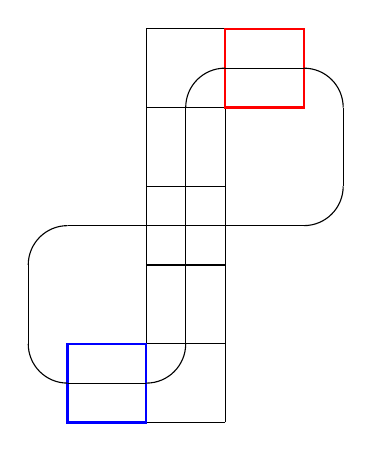
\begin{tikzpicture}
            \draw (2,0) grid (3,5);
            
            \draw[blue, thick] (1,0) rectangle (2,1);
            \draw[red, thick] (3,4) rectangle (4,5);

            \draw[color=black] (1,0.5) -- (2,0.5);
            \draw[color=black] (0.5,1) -- (0.5,2);
            \draw[color=black] (2.5,1) -- (2.5,4);
            \draw[color=black] (1,2.5) -- (4,2.5);
            \draw[color=black] (3,4.5) -- (4,4.5);
            \draw[color=black] (4.5,3) -- (4.5,4);

            \draw[color=black] (0.5,1) to[in=180,out=270] (1,0.5);
            \draw[color=black] (2,0.5) to[in=270,out=0] (2.5,1);
            \draw[color=black] (0.5,2) to[in=180,out=90] (1,2.5);
            \draw[color=black] (4,2.5) to[in=270,out=0] (4.5,3);
            \draw[color=black] (2.5,4) to[in=180,out=90] (3,4.5);
            \draw[color=black] (4.5,4) to[in=0,out=90] (4,4.5);
        \end{tikzpicture}
        }
        \caption{Reachable Cells $t=7$}
        \label{fig:ex7}
    \end{minipage}
\end{figure*}
\begin{figure*}[b]
    \lstinputlisting[caption=Incremental Approach Pathfinding, label={lst:inc_path}]{listings/inc_path.lp}
\end{figure*}

\texttt{initialstate} expresses that the earliest action may be received at timestep 1. Thus, a \texttt{starttime} can be generated for this timestep as well as the \texttt{outputaction}. The train only appears at timestep 3 with this encoding, but that can be ignored. The ability to use the earliest possible spawn time ensures that all allowed timesteps can be used for the approach.\\

The transformation to Flatland actions detailed in \ref{lst:grid_out} receives the previously described \texttt{state}, \texttt{starttime}, and input predicates. These predicates encode the map and valid plans for all agents. The Listing uses \texttt{action} instead of \texttt{outputaction}, which is an abbreviation for the sake of readability.

First, \texttt{starttime} generates the spawning action (Line 1). A \texttt{stop} action is required whenever an agent starts to remain at a cell. Thus, whenever an agent remains at a cell and was at a different cell previously, a \texttt{stop} action (Action 4) is generated (Line 3). As detailed in the Flatland section, a train continues to wait until another action is given. Thus, this one action is enough. This action is also generated if no previous state exists and thus stops the automatic movement if the plan requires waiting at the spawn.

To give a short example of this behavior:

\begin{verbatim}
state(0,((4,1),"E"),1).
starttime(0,1).
state(0,((4,1),"E"),2).
state(0,((4,1),"E"),3).
...
outputaction(0,2,1).
outputaction(0,4,2).
\end{verbatim}

These states would require a \texttt{stop} action, so the train does not move automatically after the first state.

A turn is only required if more than one option exists and the agent changes directions. Otherwise, a \texttt{forward} action (Action 2) or simply continuing to move along the path would be enough. Thus, an action to turn is generated at a state with multiple choices if a direction change is performed towards the next state. Depending on the direction change, a \texttt{left} action (Action 1) or a \texttt{right} action (Action 3) is generated (Lines 5-6).

Lastly, if an agent stopped, it needs to start moving again at some point. Thus, if two consecutive states with the same cell are followed by a state at another cell, an action is required. In this case, a \texttt{forward} action is generated (Line 10). It is not generated if the change of position already entails a turn which fulfills the conditions above. This action is enough to continue the movement. Thus, no \texttt{forward} action is required.\\

The advantage of this encoding is its simplicity, which makes it easy to extend. However, grounding is the limiting factor, with the main factors being the representation of the paths and the enforcement of constraints. Both are inefficient in this approach and the main targets for optimization in the following approaches.

\subsection*{Incremental}
\begin{figure*}[t]
    \lstinputlisting[caption=Incremental Approach Constraints, label={lst:inc_sched}]{listings/inc_scheduling.lp}
    \lstinputlisting[caption=Incremental Approach Check, label={lst:inc_check}]{listings/inc_check.lp}
\end{figure*}
\begin{figure*}[b]
    \lstinputlisting[caption=Grid to Graph Conversion, label={lst:graph_conv}]{listings/graph_conversion.lp}
\end{figure*}

Not every timestep defined by the earliest start and latest arrival time is necessary to solve the problem. This approach reduces grounding by minimizing the necessary timesteps. To that end, grounding and solving are done incrementally until a solution is found.\\

In its structure, it imitates the grid approach, yet only one timestep is grounded at a time. Before continuing, the solvability of the current grounded rules is checked. If no solution exists, the next timestep is grounded on top of it and the cycle continues. The process can be seen in Figure \ref{fig:ex1}, \ref{fig:ex2} and \ref{fig:ex7}.

The modified pathfinding is shown in Listing \ref{lst:inc_path} and very similar to the grid approach. Instead of grounding rules for a variable $T$, the grounding depends on a set $t$. This $t$ starts at 1, is set by the iteration and used to control grounding. All rules work the same as in the grid approach, except the generation of \texttt{starttime} (Line 1). As no information about future timesteps exists, it is impossible to ensure that only one \texttt{starttime} holds per train. Therefore, this is enforced later and \texttt{starttime} may be generated for every timestep as of now. The rule enforcing the horizon from the grid approach is not used herein, as it is not necessary. This encoding always finds the best solution, but it has to be noted that it uses a global horizon instead of the individual horizons.

In the first iteration, only input and the rules from $t=1$ are grounded. For Figure \ref{fig:example}, this leads to the following grounded predicates (the reachable cells are visualized in Figure \ref{fig:ex1}), as all further grounding would require a larger $t$:

\begin{small}
\begin{verbatim}
starttime(0,1)
\end{verbatim}
\end{small}

With additional grounding for $t=2$ (the reachable cells are visualized in Figure \ref{fig:ex1}) the grounded predicates would contain:

\begin{small}
\begin{verbatim}
starttime(0,1).starttime(0,2).
state(0,((4,1),"E"),2).
\end{verbatim}
\end{small}

An additional iteration with $t=3$ would lead to the following grounded predicates:

\begin{small}
\begin{verbatim}
starttime(0,1).starttime(0,2).starttime(0,3).
state(0,((4,1),"E"),2).state(0,((4,1),"E"),3).
state(0,((4,2),"E"),3).
\end{verbatim}
\end{small}

This illustrates the nature of grounding. The interdependencies are not represented in the examples above, but the predicates show how grounding generates every possible predicate. The predicates above can be understood as the nodes in a graph, connected through logical rules. For example, a solution cannot contain \texttt{state(0,((4,1),"E"),2)} without \texttt{starttime(0,1)}. The second predicate \texttt{state(0,((4,1),"E"),3)} could be generated by another \texttt{starttime} or by waiting at the start cell.\\

This cycle of grounding continues until a valid solution can be found. As of now, every solution is a valid one, so the encoding would terminate directly after $t=1$. The constraints are formulated in Listing \ref{lst:inc_sched} and \ref{lst:inc_check}.

Listing \ref{lst:inc_sched} contains constraints, which can be directly checked while grounding timesteps $t$. Vertex conflicts (Line 3) and swap conflicts (Line 5) are forbidden in the same way as they were in the grid approach, but enforced only for the current $t$. Therefore, no new states and interdependencies which lead to conflicts are grounded. The goal predicate is generated for every $t$ as well.

After every grounded timestep, but before solving, global constraints (constraints requiring all timesteps) are grounded to check for solvability. Unlike the sections controlled by $t$, this grounding is not reused. Instead, it has to be repeated for every added timestep, as it depends on all predicates grounded before. These rules can be found in Listing \ref{lst:inc_check}. Therein, the goal condition is enforced (Line 3), similarly as in the grid approach. It also enforces that only one \texttt{starttime} holds per train (Line 1). This is necessary due to the structure changes mentioned above.\\

This approach reduces grounding in most cases, but increases solving time, as it solves repeatedly and unsatisfiability is not always efficiently determined. Ensuring a grounded program is unsatisfiable might require a complete search, depending on the program. For this encoding to be an improvement, the time saved by the reduced grounding must surpass the additional solving time. The experiment section will show that it does not.

An advantage of this approach is that it does not require an estimate for the horizon. Yet, it also uses a global horizon instead of the individual horizons, as specified by Flatland.

\subsection*{Graph}
\begin{figure*}[t]
\begin{minipage}[t]{0.45\textwidth}
    \centering
    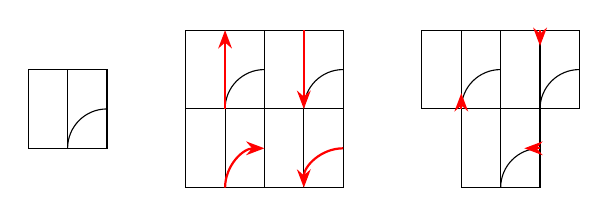
\begin{tikzpicture}
        \draw (0,0.5) rectangle (1,1.5);
        \draw (0.5,0.5) -- (0.5,1.5);
        \draw (0.5,0.5) to[out=90,in=180] (1,1);

        \draw (2,0) grid (4,2);
        \draw (2.5,1) to[out=90,in=180] (3,1.5);
        \draw[-{Stealth},color=red,thick] (2.5,1) -- (2.5,2);
        \draw (3.5,1) to[out=90,in=180] (4,1.5);
        \draw[-{Stealth},color=red,thick] (3.5,2) -- (3.5,1);
        \draw (2.5,0) -- (2.5,1);
        \draw[-{Stealth},color=red,thick] (2.5,0) to[out=90,in=180] (3,0.5);
        \draw (3.5,0) -- (3.5,1);
        \draw[-{Stealth},color=red,thick] (4,0.5) to[out=180,in=90] (3.5,0);

        \draw (5,1) grid (7,2);
        \draw (5.5,0) rectangle (6.5,1);
        \draw (5.5,1) -- (5.5,2);
        \draw (5.5,1) to[out=90,in=180] (6,1.5);
        \draw[-{Stealth},color=red,thick] (5.5,1) -- (5.5,1.2);
        \draw (6.5,1) -- (6.5,2);
        \draw (6.5,1) to[out=90,in=180] (7,1.5);
        \draw[-{Stealth},color=red,thick] (6.5,2) -- (6.5,1.8);
        \draw (6,0) -- (6,1);
        \draw (6,0) to[out=90,in=180] (6.5,0.5);
        \draw[-{Stealth},color=red,thick] (6.5,0.5) -- (6.3,0.5);
    \end{tikzpicture}
    \caption{Cell(1), Grid(2), Graph(3)}
    \label{fig:graph}
\end{minipage}
\begin{minipage}[t]{0.54\textwidth}
    \centering
    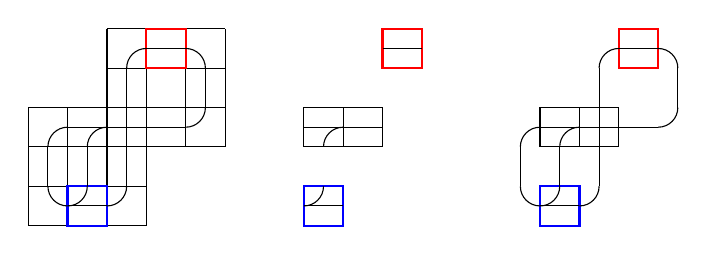
\begin{tikzpicture}
        \draw[step=0.5] (0,0) grid (1.5,1.5);
        \draw[step=0.5] (0.999,0.999) grid (2.5,2.5);
        \draw[blue, thick] (0.5,0) rectangle (1,0.5);
        \draw[red, thick] (1.5,2) rectangle (2,2.5);

        \draw (0.5,0.25) -- (1,0.25);
        \draw (0.25,0.5) -- (0.25,1);
        \draw (1.25,0.5) -- (1.25,2);
        \draw (0.5,1.25) -- (2,1.25);
        \draw (1.5,2.25) -- (2,2.25);
        \draw (2.25,1.5) -- (2.25,2);
        \draw (0.75,0.5) -- (0.75,1);

        \draw (0.25,0.5) to[in=180,out=270] (0.5,0.25);
        \draw (1,0.25) to[in=270,out=0] (1.25,0.5);
        \draw (0.25,1) to[in=180,out=90] (0.5,1.25);
        \draw (2,1.25) to[in=270,out=0] (2.25,1.5);
        \draw (1.25,2) to[in=180,out=90] (1.5,2.25);
        \draw (2.25,2) to[in=0,out=90] (2,2.25);
        \draw (0.5,0.25) to[in=270,out=0] (0.75,0.5);
        \draw (0.75,1) to[in=180,out=90] (1,1.25);


        \draw (3.5,0) rectangle (4,0.5);
        \draw (4,1) rectangle (4.5,1.5);
        \draw (4.5,2) rectangle (5,2.5);
        \draw (3.5,0) rectangle (4,0.5);
        \draw (3.5,1) rectangle (4,1.5);
        \draw[blue, thick] (3.5,0) rectangle (4,0.5);
        \draw[red, thick] (4.5,2) rectangle (5,2.5);

        \draw (3.5,0.25) -- (4,0.25);
        \draw (3.5,1.25) -- (4.5,1.25);
        \draw (4.5,2.25) -- (5,2.25);

        \draw (3.5,0.25) to[in=270,out=0] (3.75,0.5);
        \draw (3.75,1) to[in=180,out=90] (4,1.25);


        \draw (6.5,0) rectangle (7,0.5);
        \draw (7,1) rectangle (7.5,1.5);
        \draw (7.5,2) rectangle (8,2.5);
        \draw (6.5,1) rectangle (7,1.5);
        \draw[blue, thick] (6.5,0) rectangle (7,0.5);
        \draw[red, thick] (7.5,2) rectangle (8,2.5);

        \draw (6.5,0.25) -- (7,0.25);
        \draw (6.25,0.5) -- (6.25,1);
        \draw (7.25,0.5) -- (7.25,2);
        \draw (6.5,1.25) -- (8,1.25);
        \draw (7.5,2.25) -- (8,2.25);
        \draw (8.25,1.5) -- (8.25,2);
        \draw (6.75,0.5) -- (6.75,1);

        \draw (6.25,0.5) to[in=180,out=270] (6.5,0.25);
        \draw (7,0.25) to[in=270,out=0] (7.25,0.5);
        \draw (6.25,1) to[in=180,out=90] (6.5,1.25);
        \draw (8,1.25) to[in=270,out=0] (8.25,1.5);
        \draw (7.25,2) to[in=180,out=90] (7.5,2.25);
        \draw (8.25,2) to[in=0,out=90] (8,2.25);
        \draw (6.5,0.25) to[in=270,out=0] (6.75,0.5);
        \draw (6.75,1) to[in=180,out=90] (7,1.25);

    \end{tikzpicture}

    \caption{Vertex Reduction}
    \label{fig:reduction}
\end{minipage}
\end{figure*}
\begin{figure*}[b]
    \lstinputlisting[caption=Weighted Approach Graph Transformation, label={lst:weight_red}]{listings/weighted_reduction.lp}
\end{figure*}

This encoding transforms the grid to a directed graph, which serves as a basis for further abstractions and allows for easier application of strategies developed for graphs. Following approaches are going to use this transformation. The transformation is not necessary to implement them, but it helps with applying and understanding them, thus its detailed it here.\\

The main change can be summarized as separating information. Until now, transition represented the position, where the agents may be, as well as the allowed movements. That information is now split into vertices and edges.

The transformation is detailed in Listing \ref{lst:graph_conv}. Every transition $t = ((x,y),(\mathit{d1},\mathit{d2}))$ is simplified into a vertex $v = ((x,y),\mathit{d1})$ (Line 1). This representation omits the leaving directions, which can be determined by the entering direction of the next vertex. Yet, as movement is now represented by edges, it is not necessary. Multiple vertices still refer to the same cell, as did transitions.

An example of this transformation can be found in Figure \ref{fig:graph}. The leftmost cell shows the rail section, the middle cells show the representation we used up to now, which is the same as Flatland uses. The rightmost cells show the new representation used by the graph. Every cell therefore maps to at most four representations instead of previously 12. That, however, does not reduce grounding, as the reduced information is represented in the edges.

Edges are generated as follows: For each interconnected pair of transitions $(u,v)$, a new edge $e = (u,v)$ is generated (Line 3). The resulting graph is directed and retains all information. Theoretically, an undirected graph would also be feasible, as two edges always map to one rail direction. In Figure \ref{fig:graph} for example, the transitions from North to South and South to North refer to the same rail. As an undirected approach would require the facing direction of agents to be tracked separately and does not pose a clear advantage, I decided against implementing it.

For generating valid paths and scheduling them, this approach uses the exact same timestepped strategy as the grid approach. Therefore, I am not going to detail this implementation here. It can nonetheless be found on GitHub, since I implemented it to prove this approach works.\\

Compared to the grid approach, this encoding does not pose any advantages other than enabling more abstract extensions. It suffers the same complexity as the grid approach and actually performs worse due to the added overhead of transformation. Hence, it is not evaluated in the experiment section.

\subsection*{Weighted Graph}
\begin{figure*}[t]
    \lstinputlisting[caption=Weighted Approach Pathfinding, label={lst:weight_path}]{listings/weighted_path.lp}
\end{figure*}
\begin{figure*}[b]
    \lstinputlisting[caption=Weighted Approach Scheduling, label={lst:weight_sched}]{listings/weighted_scheduling.lp}
\end{figure*}

Not all vertices and edges are necessary to solve the problem. This approach reduces grounding by removing redundant vertices and edges from the graph. To that end, all vertices that don't require decisions or collision handling are cut from the graph and their edges combined into weighted edges.\\

That is achieved by transforming the graph generated by the previous approach before computing solutions on it. The new vertices are starts, goals, decision vertices and crossings. This is shown in the rightmost section of Figure \ref{fig:reduction}, where the finished representation is shown. This is the same example as before but was extended to contain decision vertices.

The new vertices are identified by Lines 1-3 in Listing \ref{lst:weight_red}. Crossings or decisions (Line 1), starts (Line 2) and goals (Line 3) constitute the new edges. Crossings and decision vertices are determined by the number of vertices used to represent a cell (remember graph representation in Figure \ref{fig:graph}). A single rail in a cell, is represented by two vertices, one for each direction. Thus, additional vertices either encode a decision or a crossing.

For generating the weighted edges, an auxiliary predicate \texttt{path} is used, representing the paths between the new vertices. It encodes start, end, length, the vertex after the start, and the vertex before the end of the corresponding path. This information is encoded in predicates \texttt{edge(U,V,N,F,L)} respectively. The start $U$, end $V$, and length $N$ will constitute the new weighted edges. $F$ and $N$ are used to determine whether two weighted edges share the same rail.

The \texttt{path} predicates are generated incrementally. First, every outgoing edge of the new vertices is selected (Line 5). This encodes the information represented in the middle state of Figure \ref{fig:reduction}. Then follows the unification, where paths are extended until a new vertex is reached (Line 7). As ASP is monotonic, previous information cannot be invalidated. Therefore, a new predicate \texttt{remove} is introduced to mark previous incomplete iterations of a \texttt{path}, whenever it is extended (Line 8). This process is straightforward, as no decisions are involved. In the end, predicates \texttt{weighted\_edge(U,V,N,D)} are generated from all unremoved paths. An unremoved path $u_1,...,u_n$ would constitute a weighted edge $e = (u_1,u_n,n)$, where the weight equals the number of unified edges. The new weighted edges contain a direction $D$ as well. This indicates the first necessary direction change to follow this edge and is important for generating Flatland actions (especially the turns), but can be ignored otherwise.

The last step of the graph transformation is determining shared resources of edges. To that end, a predicate \texttt{opposed\_edge} is generated for all paths whose second vertices and before last vertices share the same cells (Line 12-16). Figure \ref{fig:reduction} shows the necessity of this. Two paths connect the middle and the goal cell. Without considering vertices on the path, both edges would be identified as triggering a swap conflict, even though they can be used simultaneously. For this identification, it would have been enough to check if any vertices on the path match (except start and end). Yet, grounding works better with a set number of comparisons than with a variable one, where every possible comparison would need to be grounded.\\

The path generation is still timestepped and follows the same concepts as before. It is handled by Listing \ref{lst:weight_path}. A \texttt{move} predicate is introduced to determine which edge an agent selects. This is necessary as the edges are weighted and paths are not represented for every timestep. First, a \texttt{starttime} is selected as in the grid approach (Line 1). This automatically generates the first state of a train (Line 2). For every state, a train may generate a \texttt{move}, which encodes a valid edge for the agent to follow (Line 4). If no \texttt{move} is generated the train stays at its position (Line 5). Otherwise, it executed the movement and generates a new state (Line 6). This continues for every agent until either its horizon or target is reached. Bot needs to be enforced when generating moves or waiting. Otherwise, these rules would create endless states to ground.\\

Constraints are enforced similarly in Listing \ref{lst:weight_sched}. It enforces that every agent must reach its goal on time (Line 1-2), that no agents may share a cell at any timestep (Line 4), and uses the \texttt{opposed\_edge} predicate to forbid swapping along the weighted edges (Line 6). The last constraint is achieved by blocking other agents from selecting an edge to move, while another agent traverses an opposed one.

A valid example of a path (only stating \texttt{move} and \texttt{starttime} predicates) in a similar scenario as before might be:

\begin{verbatim}
starttime(0,1).
move(0,(((4,1),"E"),((2,2),"N"),3,"E"),2).
move(0,(((2,2),"N"),((0,3),"E"),3,"N"),5).
\end{verbatim}

\begin{figure*}[b]
    \lstinputlisting[caption=Path Assigning Approach Pathfinding, label={lst:assign_path}]{listings/assign_path.lp}
\end{figure*}
\begin{figure*}[t]
    \lstinputlisting[caption=Path Assigning Approach Function, label={lst:assign_py}]{listings/assign_python.lp}
\end{figure*}

Every \texttt{starttime} and \texttt{move} would generate exactly one \texttt{state} predicate in this example. This shows how the transformation reduces the number of necessary predicates. The effect is stronger for longer rails, with fewer decisions or crossings.\\

This encoding only allows waiting on the remaining vertices. This reduces the number of possible solutions, which might in turn lead to solvable instances becoming unsolvable.

To get all solutions instead, edge waiting would be necessary. This would require rules for storage (how many agents may wait on an edge) and complicate the enforcement of vertex and swap constraints. To illustrate the complexity: Every edge would need to allow as many agents to wait simultaneously as edges were unified in its creation, while enforcing constraints. That would necessitate grounding specific states of the edge and reintroduce a similar amount of grounding as was previously reduced. Therefore, I decided against it.

The reduced grounding, coupled with more complicated interdependencies, increases the importance of efficient solving. That can be seen in the section Experiments. To reduce the decisions and therefore solving time, I also implemented a version which disables waiting completely, except before spawning. This can be achieved by removing Line 5 from Listing \ref{lst:weight_path}. However, this change might not improve the solving time, as it might remove easier solutions, which can be found faster. However, it would improve scenarios, where complete searches are required.

The advantage of this encoding is the reduced grounding, which should exceed the additional overhead of transformation. A disadvantage is the increased risk of unsatisfiability by sacrificing possible solutions. Both will be evaluated in the experiment section.

\subsection*{Path assigning}
\begin{figure*}[b]
    \lstinputlisting[caption=Path Assigning Approach Scheduling and Constraints, label={lst:assign_sched}]{listings/assign_scheduling.lp}
\end{figure*}

All previous approaches grounded paths for every train. Yet Flatland only has a limited number of start and goal cells. If we take our example (Figure \ref{fig:example}) and imagine that multiple trains need to be scheduled, every new train would have all possible paths grounded. Instead, this approach grounds all paths of a start-goal combination and assigns trains with this combination to them. Thus, the number of trains would not affect grounding of paths.\\

Not every train with the same start-goal combination should take the same path. Therefore, it is necessary to generate all possible paths for every combination. This allows trains to be assigned to them instead of just grounding every possible path. To generate paths and differentiate them, these paths are generated as a nested list, where every step contains the step before it.

This generation of paths is handled by Listing \ref{lst:assign_path}. An auxiliary predicate \texttt{step(U,N,V,S)} is generated. Therein, $U$ identifies the step by encoding the start. $N$ refers to the number of steps taken so far. $V$ is the current vertex. Lastly, $S$ is the step, taken before this step.

These steps are generated incrementally, starting from every start vertex (Line 1). They continue until a cycle would be generated (Line 2). Whether a cycle would be generated, is checked by a Python function (shown in Listing \ref{lst:assign_py}). The function interprets the nested list of previous steps as a string and checks if the string of the new vertex is already included. If so, this would amount to a cycle and is forbidden. I found cycles to be an easier criterion for limiting the generated paths than the highest horizon of a train starting at the corresponding start. Using cycles instead only depends on the map and did not lead to additional unsolvable instances when testing.

After all possible paths are encoded as \texttt{step} predicates, only those that form a path to a goal are selected (back in Listing \ref{lst:assign_path} Line 4). These selected steps are encoded via \texttt{path(I,N)} predicates. $I=(U,G,S)$ is a unique identifier for a path from $U$ to $G$ with the nested list of steps $S$. $N$ encodes the length of the path.

Lastly, after valid paths are determined, the information from the nested lists is extracted. The encoding follows the nested list, starting with the end (Line 6) and extracts the contained vertices (Line 7). This information is then represented by another predicate \texttt{path(I,N,V)} which encodes the same $I$ and $N$ as before and a valid vertex $V$ (Line 9). This can be described as a list of all vertices, corresponding to a path with identifier $I$.

This already complicated generation of steps would be a lot more complicated if waiting were allowed. Thus, I decided against it for now. I would have implemented if the approach had proved efficient without it, but it did not, as will be seen in the experiment section.\\

Listing \ref{lst:assign_sched} shows the scheduling and enforcement of constraints. Every train gets assigned to a valid path, which reaches the goal on time (Line 1). This automatically enforces the goal and the individual horizon. 

Vertex and swap conflicts are handled for the paths. A predicate \texttt{block(I1,I2,N)} is generated, if paths $\mathit{I1}$ and $\mathit{I2}$ would conflict, if two trains were assigned to them with a time difference of $N$ (Line 3-4). Assignments to these paths with this time difference are thus forbidden (Line 6).\\

Overall this solves examples like Figure \ref{fig:example} well with many trains. However, instead of just grounding all possible paths, it generates all possible paths while solving as well. To provide a quick example: In a scenario where a train has two possible paths, both were possible in previous approaches, but only one would be generated as true predicates. This approach instead generates both as true predicates. This is not inherently problematic as solving is efficient as long as no decision needs to be made. The complete generation of all paths does not require such. However, grounding and solving is optimized in most ASP derivates and having everything hold in solving might impact this optimization.

Using the nested list and a Python function, which must be called while grounding, might also negatively affect the encoding's performance.

The main advantage of reduced grounding only applies if the number of trains exceeds the number of start-goal combinations. To give an estimate for the grounding: The same start can have different starting directions, every start therefore counts as two starts in complexity. Two starts and goals would thus equal $2 \times 4 = 8$ combinations to generate paths for.

Therefore, instances with more trains than start-goal combinations could profit from this implementation, but there are many possible problems.

\subsection*{Ordered}
\begin{figure*}[t]
    \lstinputlisting[caption=Ordered Approach Pathfinding, label=lst:ord_path]{listings/ordered_path.lp}
    \lstinputlisting[caption=Ordered Approach Scheduling, label=lst:ord_sched]{listings/ordered_scheduling.lp}
\end{figure*}
\begin{figure*}[b]
    \begin{minipage}[b]{0.39\textwidth}
        \centering
        \scalebox{0.6}{
        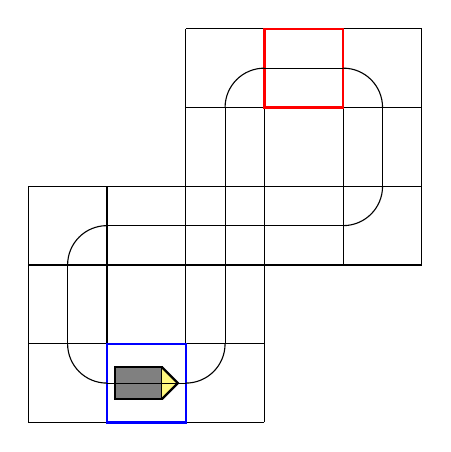
\begin{tikzpicture}
            \draw[step=1] (0,0) grid (3,3);
            \draw[step=1] (1.998,1.998) grid (5,5);

            \draw[thick, fill=black!50] (1.1,0.3) -- (1.7,0.3) -- (1.7,0.7) -- (1.1,0.7) -- cycle;
            \draw[thick, fill=yellow!50] (1.7,0.7) -- (1.9,0.5) -- (1.7,0.3);
            
            \draw[blue, thick] (1,0) rectangle (2,1);
            \draw[red, thick] (3,4) rectangle (4,5);

            \draw[color=black] (1,0.5) -- (2,0.5);
            \draw[color=black] (0.5,1) -- (0.5,2);
            \draw[color=black] (2.5,1) -- (2.5,4);
            \draw[color=black] (1,2.5) -- (4,2.5);
            \draw[color=black] (3,4.5) -- (4,4.5);
            \draw[color=black] (4.5,3) -- (4.5,4);

            \draw[color=black] (0.5,1) to[in=180,out=270] (1,0.5);
            \draw[color=black] (2,0.5) to[in=270,out=0] (2.5,1);
            \draw[color=black] (0.5,2) to[in=180,out=90] (1,2.5);
            \draw[color=black] (4,2.5) to[in=270,out=0] (4.5,3);
            \draw[color=black] (2.5,4) to[in=180,out=90] (3,4.5);
            \draw[color=black] (4.5,4) to[in=0,out=90] (4,4.5);
        \end{tikzpicture}
        }
        \caption{Example Again}
        \label{fig:example_again}
    \end{minipage}
    \begin{minipage}[b]{0.6\textwidth}
        \centering
        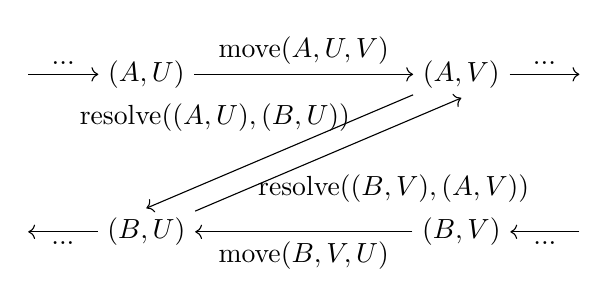
\begin{tikzpicture}[node distance=2cm, auto]
            \node (AU) at (0, 2) {$(A,U)$};
            \node (AV) at (4, 2) {$(A,V)$};
            \node (BU) at (0, 0) {$(B,U)$};
            \node (BV) at (4, 0) {$(B,V)$};

            \draw[->] (AU) -- (AV) node[midway, above] {move$(A,U,V)$};
            \draw[->] (BV) -- (BU) node[midway, below] {move$(B,V,U)$};
            \draw[->] (AV) -- (BU.north) node[pos=0.2, left] {resolve$((A,U),(B,U))$};
            \draw[->] (BU) -- (AV.south) node[pos=0.2, right] {resolve$((B,V),(A,V))$};

            \draw[->] (-1.5, 2) -- (AU) node[midway, above] {...};
            \draw[->] (AV) -- (5.5, 2) node[midway, above] {...};
            \draw[->] (BU) -- (-1.5, 0) node[midway, below] {...};
            \draw[->] (5.5, 0) -- (BV) node[midway, below] {...};
        \end{tikzpicture}
        \caption{Lock Example}
        \label{fig:lock}
    \end{minipage}
\end{figure*}
\begin{figure*}[t]
    \lstinputlisting[caption=Ordered Approach Extracting States, label=lst:ord_states]{listings/ordered_states.lp}
\end{figure*}

Timesteps, which all previous approaches used, are the greatest factor when it comes to grounding. This approach tries to implement a solving strategy without them. To that end, it replicates the method described in \cite[Behrens et al. 2023]{Behrens2023} and applies it to Flatland. The concept is to generate timestep-free paths for all trains and then schedule them to enforce the constraints.\\

Paths are encoded as a selection of edges for each train. Every selection has to map to exactly one possible path. Therefore, cycles are disallowed, as differentiating would require reintroducing timesteps or something of similar efficiency. This generation of paths reduces the search space without impacting solvability.

These paths are generated in Listing \ref{lst:ord_path}. The edges taken by agents are encoded as \texttt{move} predicates. First, two moves are generated for entering (from "Start") and leaving (to "End") the map (Lines 1-2). These moves are then connected by a set of moves. Every vertex may have up to one move leaving it (Line 4). If a vertex is left by a move it must not have more than one entering it (Line 9). To form a valid path, every move which does not start at "Start" needs to have a previous move (Line 6) and every move, which does not end at "End", has to have a follow-up move (Line 7). To give a short example of a valid move for the scenario in Figure \ref{fig:example_again}:

\begin{verbatim}
move(0,"Start",((4,1),"E")).
move(0,((4,1),"E"),((4,2),"E")).
move(0,((4,2),"E"),((3,2),"N")).
move(0,((3,2),"N"),((2,2),"N")).
move(0,((2,2),"N"),((1,2),"N")).
move(0,((1,2),"N"),((0,2),"N")).
move(0,((0,2),"N"),((0,3),"E")).
move(0,((0,3),"E"),"End").
\end{verbatim} 

\begin{figure*}[b]
    \begin{minipage}[t]{0.32\textwidth}
        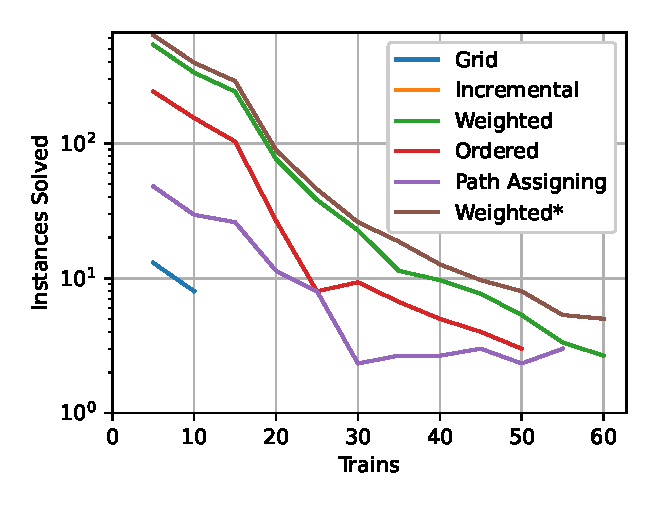
\includegraphics[width=1\textwidth]{images/sparse_s.eps}
        \caption{Sparse Domain}
        \label{fig:sparse}
    \end{minipage}
    \begin{minipage}[t]{0.32\textwidth}
        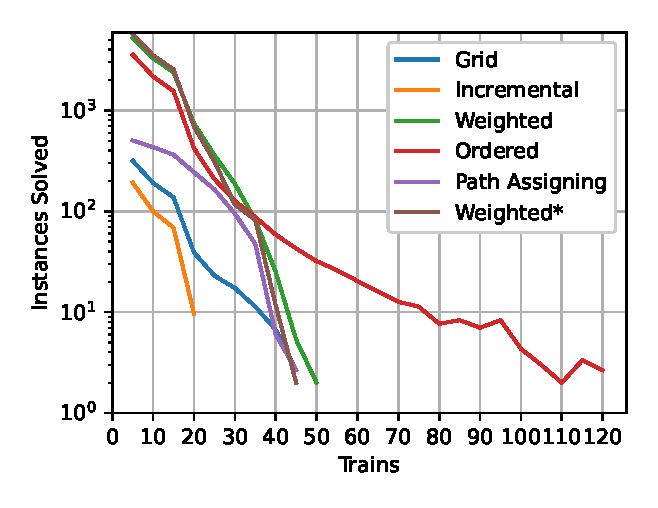
\includegraphics[width=1\textwidth]{images/normal_s.eps}
        \caption{Mean Domain}
        \label{fig:middle}
    \end{minipage}
    \begin{minipage}[t]{0.32\textwidth}
        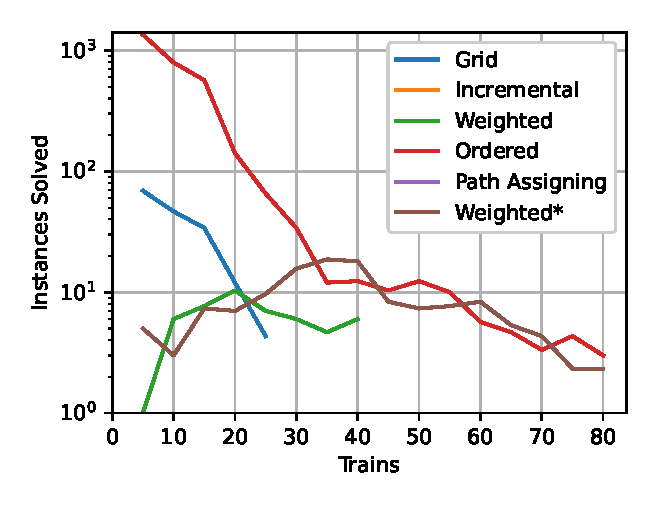
\includegraphics[width=1\textwidth]{images/dense_s.eps}
        \caption{Dense Domain}
        \label{fig:dense}
    \end{minipage}
\end{figure*}

Valid paths are always generated. The start move always holds, and as a cycle is impossible (for example another move to $(4,1)$), the only way to end the path is by reaching the goal. Cycles might form on the rest of the map, but they can be ignored, as removing them would be more resource-intensive.\\

These paths are then scheduled in Listing \ref{lst:ord_sched}. To preserve the advantages of an approach without timesteps, they must not be reintroduced for enforcing constraints. Therefore, an abstract predicate \texttt{resolve((A,U),(B,V))} is introduced (Line 1). It is generated whenever two moves to the same cell hold for different agents. It expresses that $A$ has to leave $U$ before or at the same time as $B$ enters $V$. The reverse can also be generated. This predicate automatically guards against vertex conflicts.

Swap conflicts are a subgroup of locked situations in this structure. Those are situations where agents cannot move, as every agent waits for another to pass first. These situations are forbidden by the rule \texttt{\#edge} (Line 3-4). \texttt{move} and \texttt{resolve} predicates constitute a new graph, where agent $A$ and vertex $U$ form a vertex $(A,U)$ and the predicates connect them. \texttt{resolve((A,U),(B,V))} does not constitute an edge between $(A,U)$ and $(B,V)$ but instead between the vertex before $A$ reached $U$ and $(B,V)$. An example of the resulting graph for a swap conflict can be seen in Figure \ref{fig:lock}. This Figure is a simplification. $U$ and $V$ are placeholders for vertices, which refer to the same cell. Thus, $(A,U)$ and $(B,U)$ refer to the same cell, but $U$ can stand for different vertices. The Figure shows that locked situations form cycles on the new graph. \texttt{\#edge} simply forbids cycles on the graph it received.

The remaining problem is the enforcement of the horizons. I did not find a way of handling them without reintroducing timesteps. Grounding every possible timestep would lead back to a similar complexity as that of the grid approach, thus offering no advantages. Therefore, I will keep this encoding without the enforcement of individual horizons.\\

This encoding encodes paths vastly different from the previous approaches, which were easily converted into actions for Flatland. Therefore, these paths have to be brought back into a timestepped format for conversion. This differs from searching for valid paths, as it is just a conversion of a predetermined solution. This is handled in Listing \ref{lst:ord_states}, which is not another section of the encoding. Instead, it computes the states for a predetermined solution separately, depending on the previously generated path.

This implementation fills the new graph with timesteps. Whenever a resolve needs an agent to arrive at a later time, the timestep for this vertex is updated if the new time exceeds the previous. This continues until no changes occur. First, every agent starts despawned at the earliest possible timestep (Line 1). This is encoded in \texttt{tstate(A,V,T)} as agent $A$ is at vertex $V$ at timestep $T$. For every \texttt{tstate} with a compatible \texttt{move}, the next \texttt{tstate} is generated (Line 3). If an agent resolves first at a cell, the other agent may only pass after the first has left. Thus, a \texttt{tstate} is generated for the second agent after the first passed (Line 4). In this way, multiple timesteps for every agent and vertex combination are generated. For every agent and vertex, the tstate with the highest timestep is selected. These tstates constitute a valid and optimal plan that obeys the \texttt{resolve} predicates (Line 6). This leaves some gaps, which are filled with states to represent waiting (Line 8). The result is similar to states generated by the grid approach, and can be converted into Flatland actions.\\

The resulting encoding efficiently generates plans without timesteps. But the lack of enforcing horizons leads to a varying violation thereof. Therefore, it is not applicable to the task at hand. This encoding is useful to efficiently prove solvability under the given constraints and could therefore be used to reason whether an instance would be solvable without horizons.

\begin{figure*}[t]
    \begin{minipage}[t]{0.32\textwidth}
        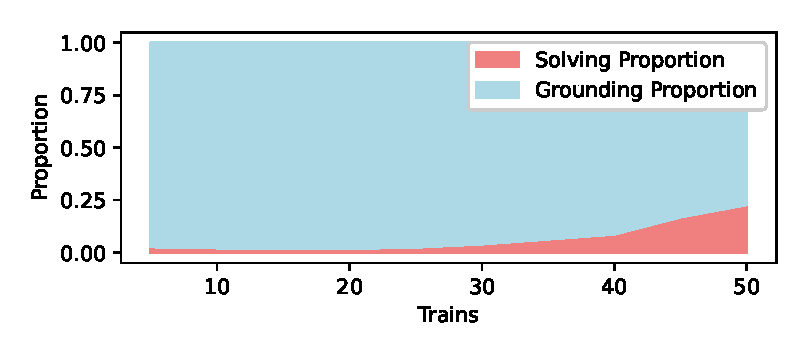
\includegraphics[width=1\textwidth]{images/weighted_s.eps}
        \caption{Weighted Solving Percentage}
        \label{fig:weighted}
    \end{minipage}
    \begin{minipage}[t]{0.32\textwidth}
        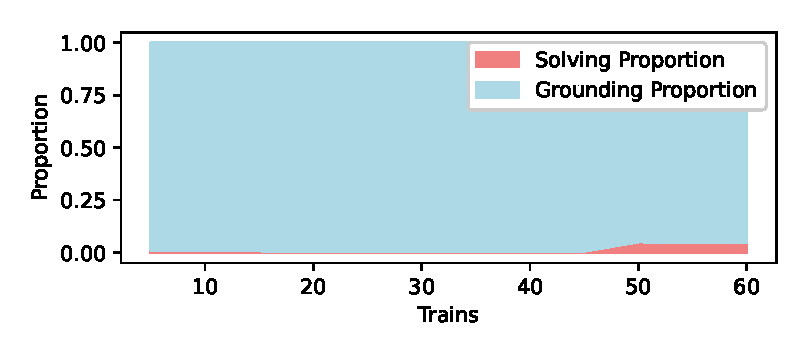
\includegraphics[width=1\textwidth]{images/weighted_reduced_s.eps}
        \caption{Weighted* Solving Percentage}
        \label{fig:weighted*}
    \end{minipage}
    \begin{minipage}[t]{0.32\textwidth}
        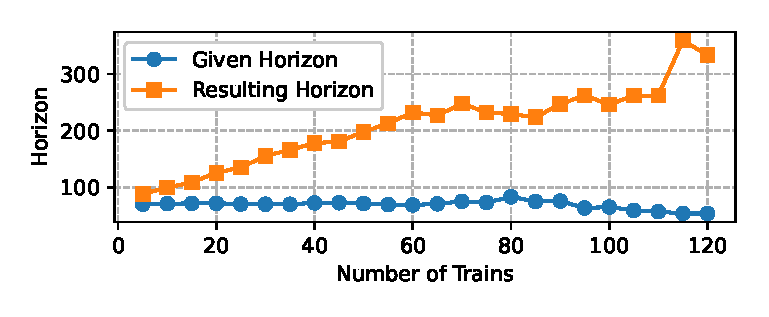
\includegraphics[width=1\textwidth]{images/horizons.eps}
        \caption{Ordered Approach Horizons}
        \label{fig:horizon}
    \end{minipage}
\end{figure*}

\section*{Experiments}
The evaluation was run on a single core of an AMD Ryzen 5 7600X (5.45GHz) with 4800Mhz RAM. The set limit was 20 minutes and no more than 20 GiB were allowed to be used. Within those 20 minutes, instances were solved one after another until the timeout was reached. The continuous measurement is intended to average out fluctuations, but falls short for instances with many trains, where one instance takes nearly 20 minutes and fluctuations are the norm. An encoding that fails due to memory or unsolvable instances gets two additional trials before failing completely. That was put in place to deal with Flatland's unsolvable instances as well as smooth the graphs.

Of all environments that were expressive, I evaluated the sparsest (Figure \ref{fig:sparse}), the densest (Figure \ref{fig:dense}) and a middle ground (Figure \ref{fig:middle}). The exact statistics for the generation and results can be found in the GitHub repository. \cite{Git24}\\

\section*{Discussion}
The grid approach works as a baseline, and its direct improvement, the incremental approach, does not improve it. The additional solving time of the incremental approach far exceeds the reduced grounding time. This is seen in all three environments, whereby it does not even solve one instance in the dense environment.

Without sacrificing constraints, the weighted approach is the winner of this evaluation over all three environments. Its greatest strength lies in the sparse environment. That was to be expected as the transformation of the map works best therein.

Weighted*, which refers to the same approach without waiting, improves upon that by reducing solving time. As shown in Figure \ref{fig:weighted}, the solving time made up a growing percentage in the weighted approach while it stayed relatively constant in Figure \ref{fig:weighted*}. Interestingly, fewer trains lead to fewer solved instances in the densest environment. This happens as more instances are unsolvable and the benchmark fails. The reason for this might be that Flatland calculates more optimistic horizons for fewer trains, which increases unsolvable instances. This is probable, as more trains lead to fewer unsolvable instances overall. Nonetheless, an efficient implementation of edge waiting would be a good subject for further research, in order to reduce unsolvable instances.

Path assigning is limited to sparse environments, where it beats the baseline. However, it neither reaches the same performance as weighted nor is it useful in other environments. That was to be expected, as only the sparse environment (Figure \ref{fig:sparse}) provides few start-goal combinations. In the densest environment (Figure \ref{fig:dense}), it performs even worse than the baseline, as the overhead exceeds any possible advantage with increasing trains.

The ordered approach consistently finds solutions for all environments, but is not comparable as it does so by sacrificing the horizons. Its generated horizons are worse by a wide margin as seen in Figure \ref{fig:horizon}. Finding a way to check timesteps without reintroducing timesteps would be another target for further work.\\

\section*{Conclusion}
This work shows different approaches to modelling pathfinding (specifically Flatland) problems in ASP and also evaluates their trade-offs.

The overall best encoding is the weighted one. However, this might be limited to problems from Flatland, as the encoding probably fares worse in domains without spawning. The reduction of grounding in an environment representing different points of time remains the biggest issue and none of the herein explained approaches pose a reliable solution.

Therefore, the main goal of future work would be to focus on further abstractions to reduce grounding.\\

\hrule
\section*{Content Breakdown}
\small
This work includes both a project and a bachelor thesis. The project is part of the module INF-6030 "Scientific Working" and consists of the GitHub repository \cite{Git24}, the work on interfacing Flatland with ASP, and the graph approach (as well as an additional more basic approach found in the GitHub for better understanding). The bachelor thesis consists of all advanced approaches discussed in this work and their evaluation.

\bibliographystyle{splncs04}
\bibliography{documentation}{}
\end{multicols*}
\end{document}

TODO if time (ordered by importance):
    - add step example to path_assigning
    - add choicepoint to example map
    - githbub footnotes